\documentclass{article}

\usepackage{amsmath}
\usepackage{amsthm}
\usepackage{amssymb}
\usepackage{color}
\usepackage{tikz}
\usetikzlibrary{shapes,arrows.meta,backgrounds}
\usepackage{etoolbox}
\usepackage{url} % for urls in bibliography
\usepackage[parfill]{parskip} % no paragraph indents, leave blank line
\usepackage{graphicx}
\usepackage{subcaption}
\usepackage{listings}

\graphicspath{ {./drawio/} }

% Need this to keep the space before theorems when using parfill parskip
% https://tex.stackexchange.com/questions/25346/wrong-spacing-before-theorem-environment-amsthm
\begingroup
    \makeatletter
    \@for\theoremstyle:=definition,remark,plain\do{%
        \expandafter\g@addto@macro\csname th@\theoremstyle\endcsname{%
            \addtolength\thm@preskip\parskip
            }%
        }
\endgroup

\DeclareRobustCommand{\rchi}{{\mathpalette\irchi\relax}}
\newcommand{\irchi}[2]{\raisebox{\depth}{$#1\chi$}} % inner command, used by \rchi

\title{Nitro Protocol}
\author{Tom Close}

\usepackage{mathtools}
\usepackage{bm}
\usepackage{stmaryrd} % for llbracket and rrbracket

\theoremstyle{definition}
\newtheorem{example}{Example}[section]
\newtheorem{defn}{Definition}[section]

\newcommand{\adj}[1]{\llbracket #1 \rrbracket} 
\newcommand{\enf}[1]{[#1]} 

\begin{document}

\maketitle

\section{Motivation}

A blockchain is a device that enables a group of adversarial parties to come to consensus over the contents of a shared ledger, without appealing to a trusted central authority. 
Whether using a proof-of-work or a proof-of-stake algorithm, this process has a cost both in terms of time and in terms of money.
For the Ethereum blockchain, this cost results in an effective limit of around 15 transactions per second being processed on the network.
When compared with the visa network, which can process on the order of 50,000 transactions per second, this limit supports the view that blockchains, in their current form, do not scale.

State channels offer a solution to the blockchain scaling problem.
A state channel can be thought of as a set of updatable agreements between a fixed set of participants determining how a given set of assets should be split between them.
The agreements are updated off-chain through the exchange of cryptographically signed messages between the participants according to some set of previously-agreed update rules. 
The assets in question are held in escrow on the blockchain, in such a way
that they can only be released according to the latest agreement from the state channel.
If the off-chain cooperative behaviour breaks down, for example if one party refuses to sign updates either by choice or due to unavailability, any of the parties can reclaim their share of the assets by presenting the latest agreement to the chain.
An exit game is required to give other parties the opportunity to present a later state, but all parties have the guarantee that they can reclaim their share of the funds within some finite time.

In addition to the increased throughput, state channels bring instant finality to transactions: the moment a channel update is received the participant knows that the assets transferred are now assigned to them.
They cannot access the assets immediately but they have the power to prevent any other party claiming those assets in the future.
The only requirement is that participants need to be live enough to engage in the exit game if an opponent attempts to exit an earlier state.
In practice, the requirement here is to check the chain periodically - at time intervals that are less than, but on the same order of magnitude as, the challenge duration in the exit game.

As the channel updates are created and exchanged off-chain, the channel-update throughput is limited only by the speed of constructing, signing and broadcasting the update.
Given that channel updates only needed to be communicated between participants and the system is therefore highly parallelizable, it is difficult to put a bound on the total transaction throughput of a system of state channels.
In practice the system is only limited by the on-chain operations required to move assets when opening and closing channels.

In this paper, we allow channels to be opened and closed off-chain. We enable the construction of efficient state channel networks.[TODO]

\section{Existing work}

Lightning and raiden
- payment channel networks
- directional

Celer
- directional but with multiple paths
- general conditions

Perun
- virtual payment channels (different from HTLCs)
- but using a validity time
- and then state channel networks
- constrained
[Connext - have removed the time limit with a trade-off of trusting the hub - TODO: check this]

Counterfactual
- thinks about counterfactual instantiation
- also app instance on top, which we collaborated on
- possible to do meta-channels, but the details are not given in the paper and are still being finalized

ForceMove

Our contribution:
- like perun without the time limit
Unconstrained subchannels

\section{State Channel Background}

In this paper, we are focus on the construction of networks of state channels, which we treat separately from the operation of those channels.
For the purpose of this work, we view a state channel and its states purely as a device for enabling a given party to realize a given outcome on-chain, in a sense that we will make precise.
In particular, we do not specify the state format, the update rules, the mechanics of on-chain challenges or how to respond to them.

The ForceMove framework is an example of a state channel framework that specifies all these details. 
The state channel networks presented here were designed to work with ForceMove and we will frequently present examples involving ForceMove channels.
That said, the techniques provided here should be applicable to any state channel framework sharing the features presented in this section.

We start the section by reviewing the properties of ForceMove that are important for Turbo and Nitro \footnote{We give a more complete recap of ForceMove in the appendix.}. 
We then introduce some concepts that will be useful later when reasoning about the correctness of our state channel networks. 

\subsection{ForceMove Channels}

A ForceMove state channel belongs to a set of \textbf{participants}, each defined by a unique cryptographic address.
The private keys corresponding to these addresses are used to sign updates to the channel.
We assume that the signature scheme is unforgeable, so that only the owner of the address has the capability to sign states as that participant.

Each channel has a \textbf{channel address} which is formed by taking the hash of the participant addresses along with a nonce, $k$, that is chosen by the participants in order to distinguish their channels from one another.
We assume that the hashing algorithm is cryptographically secure, so that it impossible for two different sets of participants to create a channel with the same address.
We also assume that the signature scheme and hashing algorithm together make it impossible to create a channel address that is the same as a participant address.
In practice, we accept that these statements will not be absolute but instead will hold with high probability.

A state channel ultimately determines the quantity of a given asset that each participant should receive.
The format that the asset quantity takes is an important consideration for a state channel.
Blockchains typically have a max integer size, $M$, meaning that a state channel on a single asset
has asset quantites in $\mathbb{Z}_M$, so that quantities above the max overflow.
Similarly the quantities for a state channel on two assets takes values in $\mathbb{Z}_M \times \mathbb{Z}_M$.
There are many other possibilities here, including having state channels on an arbitrary set of assets.
In this paper, we will simplify the explanation by only considering state channels on a single
asset, taking quantity values in $\mathbb{Z}$, thereby explicitly ignoring integer overflow issues.
We will refer to this asset as `coins'.

\subsection{Depositing, Holding and Withdrawing Coins}

In order to have value, a state channel system must be backed by assets held on-chain.
In our explanation, we assume that these funds are held and managed by a single smart contract,
which we will refer to as the \textbf{adjudicator}.
In practice, the adjudicator functionality and deposits could be split across multiple smart contracts.

We say that $\rchi$ \textbf{holds} $x$, in the case where there is a quantity of $x$ coins
locked on-chain against $\rchi$'s address.
We write this statement $\adj{\alpha_\rchi(x)}$, where the $\alpha$ denotes funds being held
and the $\adj{\quad}$ is used to indicate that the statement refers to state on the chain.
Note that in ForceMove, the only information stored on chain is the channel address and the quantity of the asset held for it - all other information resides in the off-chain states and is only visible on-chain in the case of a dispute.

The \textbf{deposit} operation, $D_\rchi(x)$, is an on-chain operation used to assign $x$ coins to channel $\chi$.
There are no restrictions on who can deposit coins into a channel - only that the
transaction must include a transfer of $x$ coins into the adjudicator.
\begin{align*}
D_\rchi(x) \adj{\alpha_\rchi(y)} = \adj{\alpha_\rchi(x + y)}
\end{align*}

In order to distribute the coins it holds, a state channel must have one or more mechanisms for
registering its \textbf{outcome}, $\omega$, on-chain.
This registration must be done in a way that ensures that at most one outcome can be registered for each channel.
In ForceMove, outcomes are registered either via an unanswered challenge or by the presentation
of a \textit{conclusion proof} - a special set of states signed by particpants indicating
that the channel has concluded, thus allowing them to skip the challenge timeout.
We write  $\adj{\beta_\rchi(\omega)}$ to represent the situation where the outcome $\omega$
has been registered on-chain for channel $\rchi$.

Once an outcome is registered on-chain, it can be used to transfer coins between addresses,
through the application of one or more on-chain operations:
\begin{align*}
O \adj{\alpha_\rchi(a + b)\beta_\rchi(\omega)} = \adj{\alpha_A(a)\alpha_\rchi(b)\beta_\rchi(\omega')}
\end{align*}
The specification of the precise format for the outcome, $\omega$, and the operations, $O$,
will be given in the sections on Turbo and Nitro.
In the equation above, $A$ could be either a channel address or a participant address.

The \textbf{withdrawal} operation can be used to withdraw coins held at address $A$ by any
party with the knowledge of the corresponding private key. 
Note that the signature requirement coupled with the no-collision assumption means
it is only possible to withdraw from a participant address.
If $x \leq x'$ then
\begin{align*}
W_A(x) \adj{\alpha_A(x')} = \adj{\alpha_A(x'-x)}
\end{align*}
In practice the withdrawal should also specify the blockchain address where the funds should be sent.
A potential method signature is \texttt{withdraw(fromAddr, toAddr, amount, signature)}, 
where \texttt{signature} is $A$'s signature of the other parameters
\footnote{In practice, we can add the \texttt{senderAddress} to the parameters to sign,
in order to prevent replay attacks.}.

Note that, in practice, the operations $O$ and $W$ need not be separate blockchain transactions.
For example, in the ForceMove SimpleAdjudicator, funds are withdrawn directly using $\alpha_\chi$ and $\beta_\chi$;
the intermediate state, $\alpha_A$, where funds are held against a participant address never exists on-chain.

\subsection{Value}


Value

- value (unbeatable strategy for extracting at least a given total, without assuming we add funds)
- value equivalent (if two system states have the same value)
- value preserving transition
- applications change value, opening and closing an application shouldn't

- transitioning between outcomes
- rewrite rules
- channels update independently

- possible to transition between finalizable states

\subsection{Finalizable and Enabled Outcomes}

- state of a channel
- outcome is finalizable if you can register it on-chain and no-one can stop you.
- an unbeatable strategy for getting it on-chain
- series of actions

\begin{example}{The next mover in ForceMove.}
  In a ForceMove state channel with $n$ participants, if participant $p$ has just received state $\sigma_m$ with $m > n$ and it is their turn to sign state $m+1$, then we have $\enf{\sigma_m.\beta}_p$ - the state's balances $\sigma_m.\beta$ is a finalizable outcome for $p$.
  Why? To finalize this outcome $p$ can call a force-move on $\sigma_m$ and then fail to respond within
  the timeout. [The reason why ForceMove always allows a transition to a conclude state is to
  give $p$ a way of accomplishing the same outcome off-chain.]
\end{example}

\begin{example}{Two conclusion proofs.}
  In a ForceMove state channel, if two different conclusion proofs with different outcomes,
  $\beta_1 \neq \beta_2$, are both held by participants $p_1$ and $p_2$, then no outcome is finalizable by any participant.
  Why? No finalizable outcome other than $\beta_1$ is possible any party $p$, as it is always
  possible for either $p_1$ or $p_2$ to register the conclusion proof resulting $\beta_1$ immediately.
  But the same is also true for $\beta_2$. Therefore no finalizable outcome exists.
  [For this reason, participants should never sign more than one conclusion state.]
\end{example}

- enabled outcomes




\begin{example}{Pre-fund setup in ForceMove.}
  In a ForceMove state channel with $n$ participants $P$, at end of the pre-fund setup i.e.
  when the last state to be broadcast was $\sigma_n$, then we have $\enf{\sigma_n.\beta}_P$ -
  the state's balances $\sigma_n.\beta$ is finalizable for all participants of the channel.
  Why? According to the ForceMove transition rules, the outcome must remain unchanged for the
  first $2n$ states. That means that every participant must contribute another signature before
  the outcome of the state can change. By with-holding this signature and forcing the channel to
  conclusion through a series of force-moves, any participant can ensure that the current
  outcome is registered on-chain.
\end{example}

\section{Turbo Protocol}

Turbo protocol allows a set of participants who already have a funded channel to open and
close sub-channels without any on-chain transactions. 
In order to do this, the protocol specifies the format of the channel outcomes and how
they are interpreted on-chain.
It does not specify the channel update and challenge mechanics but can be combined with
ForceMove to provide a fully functional system.

As an example of what Turbo enables, suppose Alice and Bob want to play a game of chess and that
they already have an existing state channel, $\rchi_L$.
The winner of the game of chess should receive 2 coins from the loser and $\rchi_L$ currently holds
5 of Alice's coins and 5 of Bob's.

\begin{center}
  \includegraphics[scale=0.5]{turbo_start} % TODO: tikz
\end{center}

Alice and Bob proceed by creating a new channel $\rchi_C$ for the chess game with the appropriate starting state.
They then update $\rchi_L$ to allocate funds to these games.

\begin{center}
  \includegraphics[scale=0.5]{turbo_open} %TODO: tikz
\end{center}

Once the funds are allocated, they are free to play the game of chess.
Updates to the chess channel are independent from updates to $\rchi_L$ and to
any other sub-channels that are potentially funded by it. 
Alice wins the chess game, so the final state in the chess channel allocates all the
funds to her.

\begin{center}
  \includegraphics[scale=0.5]{turbo_close} %TODO: tikz
\end{center}

To close the chess channel off-chain, Alice and Bob update the state of the ledger channel to absorb the outcome of the game.

\begin{center}
  \includegraphics[scale=0.5]{turbo_finish} %TODO: tikz
\end{center}

In the rest of this section we will present the protocol that makes the above interaction
possible.

\subsection{Turbo Outcomes and Operations}

Turbo protocol specifies the interpretation of channel outcomes and the operations that
manipulate them once they are on-chain.
The process of registering the outcome with the chain is not specified, but could be accomplished
using the ForceMove protocol.

Outcomes in Turbo take the form of an ordered list of address-value pairs.
To write outcomes we will use the notation $\{a_1{:}v_1, \dots, a_n{:}v_n \}$, where the $a_i$
represent addresses and the $v_i$ represent values.
The key idea behind Turbo is that the addresses in the outcomes are not limited to being
participant addresses but that they can also be addresses of other \textit{channels}.

The ordering in the outcome is significant and is used to determine a priority order for payouts,
which becomes important if channel does not hold enough funds to cover the entire outcome.

The naive algorithm for distributing the funds is to work along the outcome from the front,
paying funds out to the corresponding address until no funds are remaining.
In practice, we avoid introducing a dependency on the order of the payouts by using
the \textbf{overlap} function $\texttt{overlap}(p, \omega, x)$, which returns the payout owed
to $p$ from outcome $\omega$ when the channel is funded with $x$.
The overlap function can be written in python as follows:

\begin{minipage}{\linewidth} % minipage to avoid page breaks
  \lstinputlisting[language=Python]{code/overlap.py}
\end{minipage}

general pattern is 
- funds deposited into a payment channel address
- an outcome assigns funds from the payment channel to 




\begin{center}
  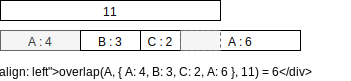
\includegraphics[scale=0.7]{overlap} % TODO: tikz
\end{center}

- once an outcome pays out, we remove the outcome

\begin{center}
  \includegraphics[scale=0.7]{remove} % TODO: tikz
\end{center}
\lstinputlisting[language=Python]{code/remove.py}


We will now introduce the three on-chain operations that drive Turbo: deposit, withdrawal,
and transfer.


The \textbf{transfer} operation, $T_{A,B}(x)$, is an instruction to transfer funds currently allocated
to address $A$ to address $B$, according to the outcome of channel $A$.

\lstinputlisting[language=Python]{code/transfer.py}

If channel $X$ holds x and the outcome of $X$ allocates $y$ to $Y$ within $x$.
- then update channel X to hold x, channel Y to hold y, and decrease the amount X allocates to Y by y

For example, 
\begin{align*}
T_{A,B}(3) \adj{\alpha_A(10)\beta_A(B: 3, C: 7)} = \adj{\alpha_A(7)\alpha_B(3)\beta_A(C: 7)}
\end{align*}

\subsubsection{Value Equivalence in Turbo}

- how can we know if two system states are value equivalent?
- in turbo it's simple: if there's any sequence of Ts that drive them to the same state
  then they're equivalent
- transfer operations commute
- if I can find one set of transfer operations they're equivalent

- funding a ledger channel - only deposit if it increases your value by the deposit amount
- opening a subchannel

\subsection{Ledger channels}

While this generalization allows for a variety of relationships between different channels,
we will focus here on a setup where a single parent channel funds one or more sub-channels
\footnote{Note that we allow the case where the sub-channels are themselves ledger channels.}.
Following the Perun paper, we will refer to this parent channel as a \textbf{ledger channel}.

- ledger channel is assumed to be running the consensus application

\subsubsection{Opening a sub-channel}

- make precise the operation we performed in the introduction, where we opened a subchannel
- here the enforcable state for $\rchi$ is assumed to be the ready-to-fund state
- doesn't matter what application is running in the channel - just what the initial balances are
\begin{align*}
  S_1 &= \adj{\alpha_L(a+b)} &&\enf{\beta_L(A: a, B: b)}_{A, B} & \\
  S_2 &= \adj{\alpha_L(a+b)} &&\enf{\beta_L(A: a, B: b)}_{A, B}&\enf{\beta_\rchi(A: a', B: b')}_{A, B} \\
  S_3 &= \adj{\alpha_L(a+b)} &&\enf{\beta_L(A: a-a', B: b-b', \rchi: a' + b')}_{A, B}&\enf{\beta_\rchi(A: a', B: b')}_{A, B}
\end{align*}
- at each point it is value equivalent for both A and B to $a$ $b$ respectively
- each step only changes one channel at a time 
- therefore we can do by single-channel-rewrite lemma

\subsubsection{Closing a sub-channel}

- closing a subchannel is similar
- hear the finalizable state is assumed to be a conclude state from the end of the channel
\begin{align*}
S_1 &= \adj{\alpha_L(x)} &&\enf{\beta_L(A: a, B: b, \rchi: a' + b')}_{A, B}&\enf{\beta_\rchi(A: a', B: b')}_{A, B}\\
S_2 &= \adj{\alpha_L(x)} &&\enf{\beta_L(A: a + a', B: b + b')}_{A, B}&\enf{\beta_\rchi(A: a', B: b')}_{A, B} \\
S_3 &= \adj{\alpha_L(x)} &&\enf{\beta_L(A: a + a', B: b + b')}_{A, B} & 
\end{align*}
where $x = a + a' + b + b'$.
- the analysis is exactly the same as in the opening case

\subsubsection{Topping up a ledger channel}

- useful to be able to top up without disturbing sub-channels supported in a ledger channel
- topping up is similar to depositing in force-move
\begin{align*}
S_1 &= \adj{\alpha_L(x)} &&\enf{\beta(A: a, B: b, \rchi: c)}_{A, B} \\
S_2 &= \adj{\alpha_L(x)} &&\enf{\beta(B: b, \rchi: c, A: a + a')}_{A, B} \\
S_3 &= D_L(a')\adj{\alpha_L(x)} &&\enf{\beta(B: b, \rchi: c, A: a + a')}_{A, B} \\
S_4 &= \adj{\alpha_L(x + a')} &&\enf{\beta(B: b, \rchi: c, A: a + a')}_{A, B}
\end{align*}
- rearrange the current outcome to put the depositor last
- note that $\nu_A(S_3) - \nu_A(S_2) = a'$ as it should be if $A$ is to deposit

\subsubsection{Partial checkout from a ledger channel}

- partial checkout is the opposite to top up
- the scenario here is two parties have a ledger channel open, supporting one or more subchannels
- participant A wants to be able to withdraw 
- this means we need to increase the value of $\alpha_A$ 
- we will assume here that we start with $\alpha_A(0)$
\begin{align*}
S_1 &= \adj{\alpha_L(x)} \quad \enf{\beta_L(B: b, A: a, \rchi: c)}_{A, B}  \\
S_2 &= \adj{\alpha_L(x)} \quad \enf{\beta_L(B: b, A: a, \rchi: c)}_{A, B} \quad \enf{\beta_{L'}(B: b, A: a - a', \rchi: c)}_{A, B}\\
S_3 &= \adj{\alpha_L(x)} \quad \enf{\beta_L(L': x-a', A: a')}_{A, B} \quad \enf{\beta_{L'}(B: b, A: a - a', \rchi: c)}_{A, B}\\
S_4 &= \adj{\alpha_L(x)\beta_L(L': x-a, A: a')} \quad \enf{\beta_{L'}(B: b, A: a - a', \rchi: c)}_{A, B}\\
S_5 &= \adj{\alpha_{L'}(x-a')\alpha_A(a')} \quad \enf{\beta_{L'}(B: b, A: a - a', \rchi: c)}_{A, B}
\end{align*}
- technique here is to create a replacement ledger channel with the updated totals and then update the 
  original channel to point here.
- in transitioning to $S_4$ we take $L$ to the chain. probably using conclude to avoid the timeout

\section{Nitro Protocol}

% \begin{table}[h]\centering
  \begin{tabular}{|l|l|l|p{5cm}|}
    \hline
    \texttt{participants} & \texttt{address[]} & $P$ & The addresses used to sign updates to the channel. \\ \hline
    \texttt{gameLibrary} & \texttt{address} & $L$ & The address of the gameLibrary, which defines the transition rules for this channel \\ \hline
    \texttt{nonce} & \texttt{unit256} & $k$ & Chosen to make the channel's address unique. \\ \hline
    \texttt{challengeDuration} & \texttt{unit256} & $\eta$ & \\ \hline
    \texttt{turnNum} & \texttt{unit256} & $i$ & Increments as new states are produced. \\ \hline
    \texttt{guarantorFor} & \texttt{address} &  & Target channel for guarantee channels. Equal to 0 for balance channels. \\ \hline
    \texttt{balances} & \texttt{(address, uint256)[]} & $\beta$ or $\gamma$ & Current \textit{outcome} of the channel. \\ \hline
    \texttt{isFinal} & \texttt{bool} & $f$ & \\ \hline
    \texttt{data} & \texttt{bytes} & $\delta$ & \\ \hline
    \texttt{v} & \texttt{uint8} & &  ECDSA signature of the above arguments by the moving participant. \\ \cline{1-2}
    \texttt{r} & \texttt{bytes32} & & \\ \cline{1-2}
    \texttt{s} & \texttt{bytes32} & & \\ \hline
  \end{tabular}
  \caption{Nitro state format}
  \label{table:force-move-state}
\end{table}


- extension to turbo. introduce a different type of outcome. allows us to support channels through
  a third party
- call these virtual channels

- example: suppose that Alice wants to play chess with Bob
- doesn't have a ledger channel open but they both have a channel open with Hugo

- how this enables a hub

- how this enables multi-hop routing

\subsection{Nitro Outcomes and Operations}

- extends turbo by adding a new type of outcome (and a new type of channel)
- refer to this as the guarantee and write this $\gamma$
- guarantee allows one channel choose to pay out for certain parts of another outcome

- finalizing is exactly the same
- guarantee channels can follow the same force-move transition rules and challenge etc.
- interpretation of the outcomes on-chain

- in explaining how this works it will be useful to introduce another operation
- cap - ensures that one allocation can't give out more to any address than another

\lstinputlisting[language=Python]{code/cap.py}

- the claim operation

\lstinputlisting[language=Python]{code/claim.py}


- [diagram]: nitro state properties


\subsubsection{Value Calculations}

\subsection{Virtual Channels}

- outline how we can use guarantee channels to create virtual channels
- the construction we will use is as follows

\begin{figure}[h]\centering
  \begin{tikzpicture}[x = 2cm, y=1cm]
    \node (expanded0) at (0, 0) { \begin{tikzpicture}[x=2.4cm, y=1cm, framed, background rectangle/.style={draw=black,dashed, rounded corners}] 
  % Specification of nodes (position, etc.)
  \node (a0) at (0,0) { $\adj{\holds{L}{x}{}, \holds{L'}{x}{}}$ };
  \node (b0) at (-1,-1) { $\finalizable{L}{\alloc{A: a, C: b}}{A, C}$ };
  \node (b1) at (1,-1) { $\finalizable{L'}{\alloc{C:a, B:b}}{B, C}$ };
  \node (g0) at (-1,-2) { $\finalizable{G}{\guar{J}{\rchi, A, C}}{A, C}$ };
  \node (g1) at (1,-2) { $\finalizable{G'}{\guar{J}{\rchi, B, C}}{B, C}$ };
  \node (j) at (0,-3) { $\finalizable{J}{\alloc{A: a, B: b, C: x}}{A, B, C}$ };
  \node (c) at (0,-4) { $\finalizable{\rchi}{\alloc{A:a, B: b}}{A, B}$ };

  \begin{scope}[-]
    \tikzstyle{every node}=[draw=none,below]
    \draw (a0) to (b0);
    \draw (a0) to (b1);
    \draw (g0) to (j);
    \draw (g1) to (j);
  \end{scope}

\end{tikzpicture}
 };
    \node[scale=0.4, rectangle, draw, dashed, rounded corners] (state0) at (3, 1.5) { 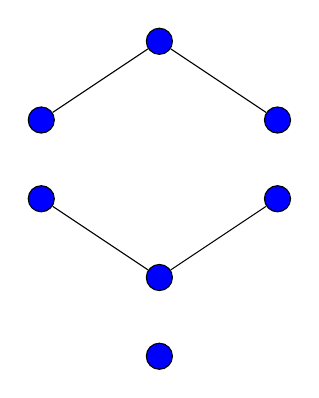
\begin{tikzpicture}[x=1.5cm,y=1cm,every node/.style={draw,solid,shape=circle,fill=blue}]

  % Specification of nodes (position, etc.)
  \node (a0) at (0,0) {};
  \node (b0) at (-1,-1) {};
  \node (b1) at (1,-1) {};
  \node (g0) at (-1,-2) {};
  \node (g1) at (1,-2) {};
  \node (j) at (0,-3) {};
  \node (c) at (0,-4) {};

  \begin{scope}[-]
    \tikzstyle{every node}=[draw,below]
    \draw[solid] (a0) to (b0);
    \draw[solid] (a0) to (b1);
    \draw[solid] (g0) to (j);
    \draw[solid] (g1) to (j);
  \end{scope}

\end{tikzpicture}
 };
    \node[scale=0.4] (state1a) at (4, 1.5) { \input{figures/virtual-channels-mini-1a} };
    \node[scale=0.4] (state1b) at (3, -1) { \input{figures/virtual-channels-mini-1b} };
    \node[scale=0.4] (state2) at (4, -1) { \input{figures/virtual-channels-mini-2} };
    \node[scale=0.4, rectangle, draw, dashed, rounded corners] (state3) at (4, -3.5) { \input{figures/virtual-channels-mini-3} };
    \node (expanded3) at (1, -6) { 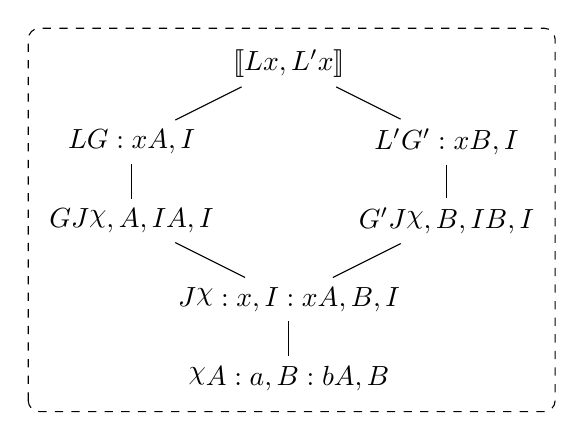
\begin{tikzpicture}[x=2cm, y=1cm, framed, background rectangle/.style={draw=black,dashed, rounded corners}] 

  % Specification of nodes (position, etc.)
  \node (a0) at (0,0) { $\adj{\holds{L}{x}{}, \holds{L'}{x}{}}$ };
  \node (b0) at (-1,-1) { $\finalizable{L}{\alloc{G: x}}{A, I}$ };
  \node (b1) at (1,-1) { $\finalizable{L'}{\alloc{G': x}}{B, I}$ };
  \node (g0) at (-1,-2) { $\finalizable{G}{\guar{J}{\rchi, A, I}}{A, I}$ };
  \node (g1) at (1,-2) { $\finalizable{G'}{\guar{J}{\rchi, B, I}}{B, I}$ };
  \node (j) at (0,-3) { $\finalizable{J}{\alloc{\rchi: x, I: x}}{A,B,I}$ };
  \node (c) at (0,-4) { $\finalizable{\rchi}{\alloc{A: a, B: b}}{A,B}$ };

  \begin{scope}[-]
    \tikzstyle{every node}=[draw=none,below]
    \draw (a0) to (b0);
    \draw (a0) to (b1);
    \draw (b0) to (g0);
    \draw (b1) to (g1);
    \draw (g0) to (j);
    \draw (g1) to (j);
    \draw (j) to (c);
  \end{scope}

\end{tikzpicture}
 };

    \begin{scope}[ultra thick]
      \tikzstyle{every node}=[below]
      \draw[-{Latex[length=3mm,width=4mm]}] (state0) edge (state1a)
                (state0) edge (state1b)
                (state1a) edge (state2)
                (state1b) edge (state2)
                (state2) edge (state3);
    \end{scope}
  \end{tikzpicture}
  \caption{Ledger channels, $x = a + b$}
  \label{fig:modes}
\end{figure} 


- worth thinking about how this works
- offload
- key is the joint A-B-C channel, source of truth for state of channel


\subsubsection{Opening a Virtual Channel}

Want to start in the situation where channels A-C and B-C exist and demonstrate how to
open the virtual channel situation

We let
\begin{align*}
l_0 &= \enf{\beta_L(A:a, C: b)}_{A, C} &
l_1 &= \enf{\beta_L(G: x)}_{A, C} \\
l'_0 &= \enf{\beta_{L'}(B:b, C: a)}_{B, C} &
l'_1 &= \enf{\beta_{L'}(G': x)}_{B, C} \\
j_0 &= \enf{\beta_{J}(A: a, B:b, C: x)}_{A, B, C} &
j_1 &= \enf{\beta_{J}(\chi: x, C: x)}_{A, B, C} \\
g &= \enf{\gamma_{G, J}(A: x, B:x, C: x)}_{A, C} &
g' &= \enf{\gamma_{G, J'}(A: x, B:x, C: x)}_{A, C} \\
v &= \enf{\beta_\chi(A: a, B: b)}_{A, B} &
\adj{S} &= \adj{\alpha_L(x)\alpha_{L'}(x)}
\end{align*}

and proceed as follows
\begin{align*}
S_1 &= \adj{S} && l_0 && l'_0 \\
S_2 &= \adj{S} && l_0 && l'_0 && g && g' && j_0 \\
S_3 &= \adj{S} && l_1 && l'_0 && g && g' && j_0 \\
S_4 &= \adj{S} && l_1 && l'_1 && g && g' && j_0 \\
S_5 &= \adj{S} && l_1 && l'_1 && g && g' && j_0 && v\\
S_6 &= \adj{S} && l_1 && l'_1 && g && g' && j_1 && v\\
\end{align*}

- first create the subchannel we want to fund
- and the joint channel and guarantee channels to support it
everything here is disconnected
- then we update the ledger channels, one at a time to fund the guarantees
- finally we update the joint channel to fund the virtual channel

\subsubsection{Closing a Virtual Channel}

Opening a channel in reverse
- start with the virtual channel coming to a finalizable outcome e.g. conclude
- then A or B propose an update to j
- once A and B have signed off, it's in C's interest too
- then they can defund the guarantee channels independently


\section{Acknowledgements}

- Andrew Stewart
- James Prestwich
- Chris Buckland
- Magmo team


\section{Appendix}

\subsection{Overview of ForceMove}
\subsection{The Consensus Game}
\subsection{Virtual Channels on Turbo}
\subsection{Payouts to Non-Participants}
\subsection{Possible Extensions}


\end{document}
